\documentclass[10pt]{beamer}

\usetheme{metropolis}
\usepackage{appendixnumberbeamer}

\usepackage{booktabs}
\usepackage[scale=2]{ccicons}

\usepackage{pgfplots}
\usepgfplotslibrary{dateplot}

\usepackage{xspace}

\usepackage{tikz}
    \usetikzlibrary{positioning}

%\usepackage{listings}
\usepackage{minted}

\usepackage{bm}%................................. Bold math symbols (after fonts)

\setbeamercolor{normal text}{bg=white}





\title{EML4930/EML6934: Lecture 02}
\subtitle{Loops, Functions, Classes, and intro to Objects}
\date{September 7, 2017}
%\author{CJ}
\author{Charles Jekel}
%\titlegraphic{\includegraphics{images/avatarCropped.png}\vspace{58cm}}
%\institute{1. University of Florida\\ 2. Stellenbosch University, South Africa}

% \titlegraphic{\hfill\includegraphics[height=1.5cm]{logo.pdf}}

\begin{document}

\maketitle

\begin{frame}{Style guide for Python}
\url{https://www.python.org/dev/peps/pep-0008/}

One thing I didn't know is that Python 3 disallows mixing tabs and spaces in your code. 

You should use spaces to denote tabs in Python.
\end{frame}

\begin{frame}[fragile]{Code blocks in C and MATLAB}
In C, code blocks are denoted with \{ and \}. In MATLAB a code block ends with an \textit{end} statement. However Python requires neither, just that the code block is indented! 
\begin{minted}
{c}
// C code
int total = 0;
for(int i=0; i<100; i++)
	{
		// curly braces indicate code block
		total += i;
	}
\end{minted}
\begin{minted}
{matlab}
% MATLAB code
total = 0
for i = 1:99
% code block starts on the line after the for loop
total = total + i;
end % statment terminates the for loop
\end{minted}

\end{frame}

\begin{frame}[fragile]{Python code for previous slide}
\begin{minted}
{python}
total = 0
for i in range(100):
    # the first code line indented begins code block
    total = total + i
# when the indentation ends, so does the code block
\end{minted}
\begin{itemize}
\item Statements clearly begin with a : in Python
\item Python forces you to indent your code blocks -- this makes Python highly readable
\item You don't need end statements in Python, instead you end the indentation block
\end{itemize}
\end{frame}

\begin{frame}[fragile]{While loop}
\begin{minted}
{python}
i = 0
while i < 10:
    print(i)
    i += 1 # this takes the previous i value and adds 1 to it
print('The while loop has finished')
\end{minted}
Notice how the format is just like a if statment. Using the : to begin the code block. The code block is indicated by the indentation. There are no end statements in Python. Rather code blocks end when the indentation is returned to normal. 
\end{frame}

\begin{frame}[fragile]{Iterating over a list}
\begin{minted}
{python}
x = [0,1,2,3,4,5,6]
for i in x:
    print(i) 
\end{minted}
\end{frame}

\begin{frame}[fragile]{Iterating over two lists}
This code simultaneously iterates over both lists
\begin{minted}
{python}
x = [0,1,2,3,4,5,6]
y = [7,8,9,10,11,12,13]
for xVal, yVal in zip(x,y):
    print(xVal, yVal) 
\end{minted}
\end{frame}

\begin{frame}[fragile]{Iterating over two lists - using range}
This code simultaneously iterates over both lists. len() tells us the length of a list.
\begin{minted}
{python}
x = [0,1,2,3,4,5,6]
y = [7,8,9,10,11,12,13]
for i in range(len(x)):
    print(x[i], y[i]) 
\end{minted}
\end{frame}

\begin{frame}[fragile]{For loop - Iterating with range()}
\begin{minted}
{python}
total = 0
for i in range(100):
    # the first code line indented begins code block
    total = total + i
\end{minted}

How range() works.
\begin{itemize}
\item for i in range(100): - iterates from 0 to 99 (100 times)
\item range(0,100) - iterates from 0 to 99 (100 times)
\item range(0,100,2) - iterates 0, 2, 4, ..., 98 (50 times)
\item range(startPoint, endPoint, stepSize) where startPoint is inclusive, endPoint is exclusive
\end{itemize}
\end{frame}

\begin{frame}[fragile]{For loop range(0,9)}
\begin{minted}
{python}
for i in range(0,9):
    '''
    this is a for loop, 
    that will print 0, 1, 2, 3, 4, 5, 6, 7, 8   
    '''
    print(i) 
\end{minted}

These are the most basic for loop. Again the : initiates the code block, and the indentation indicates the beginning and end of a code block.
\end{frame}

\begin{frame}[fragile]{Nesting a for loop}
Remember your code block is denoted with indentation in Python. 
\begin{minted}
{python}
for i in range(-10,11):
    if i < 0:
        print(i, 'is negative')
    elif i > 0:
        print(i, 'is positive')
    else:
        print(i, 'is zero')
\end{minted}
This will loop for i = -10, -9, ..., 10. Then an if-else statement is used to print whether i is negative, positive,or zero. 
\end{frame}

\begin{frame}[fragile]{Use break to \textit{break} loop}
\begin{minted}
{python}
for i in range(-10,11):
    if i == 0:
        break
    print(i)
\end{minted}

\begin{minted}
{python}
i = 0
n = 0
while i == 0:
    n += 1
    if n > 100:
        break
\end{minted}
\end{frame}

\begin{frame}[fragile]{Double nest loops}
You can double nest loops like this.
\begin{minted}
{python}
for i in range(0,10):
    for j in range(0,10):
        print(i,j)
\end{minted}
\textbf{flat is better than nested}
\begin{itemize}
\item Use functions with specific tasks to avoid a large number of nested layers
\item It is really hard to debug heavily layered code- but easy to test functions
\item Your break placement in nested code matters. Which loop are you trying to break???
\end{itemize}
\end{frame}

\begin{frame}[fragile]{Loops with the index and value - enumerate}
Often I need to create a loop through an array, where I'll need the index and value. I use enumerate() to do this.
\begin{minted}
{python}
x = [8,181,129,10,'hi']
for index, value in enumerate(x):
    # index refers to the index on the list x
    # value is the current value of x the loop is on
    print(index, value)
\end{minted}
\end{frame}

\begin{frame}[fragile]{Loops with the index and value - enumerate}
If it isn't clear, index and value can be named whatever you want.
\begin{minted}
{python}
x = [8,181,129,10,'hi']
for i,j in enumerate(x):
    print(i,j)
\end{minted}
\end{frame}

\begin{frame}[fragile]{List comprehension - basics}
This is one really neat feature in Python where you can run loops and if statements while generating a list.

List comprehension creates many Pythonic code one liners. 

An interested read \url{http://treyhunner.com/2015/12/python-list-comprehensions-now-in-color/}

\begin{minted}
{python}
x = [0,1,2,3,4,5]
y = [i**2 for i in x]
# y is a list where each item in x is squared
\end{minted}
\end{frame}

\begin{frame}[fragile]{List comprehension - more advanced}
\begin{minted}
{python}
x = [-5,-4,-3,-2,-1,0,1,2,3,4,5]
y = [i for i in x if abs(i) < 3]
# y is a list containing each item in x
# such that the absolute value of each item in x is less than 3
\end{minted}
\begin{minted}
{python}
x = [0,1,2,3,4,5]
y = [i**2 for i in x if i%2 ==0]
# y is a list where each item in x is squared
# if the item in x is an even number
\end{minted}

\begin{minted}
{python}
x = [0,1,2,3,4,5]
y = [i**2  for i in x if i**2%2 == 0]
# y is a list where each item in x is squared
# if the item squared is an even number
\end{minted}
\end{frame}

\begin{frame}[fragile]{list comprehension - multiple loops}
\begin{minted}
{python}
in : [[i,j] for i in range(2) for j in range(2)]
out: [[0, 0], [0, 1], [1, 0], [1, 1]]

in : # this is a triple nested for loop creating a list!
[[i,j,k] for i in range(2) for j in range(2) for k in range(2)]
out: [[0, 0, 0],
 [0, 0, 1],
 [0, 1, 0],
 [0, 1, 1],
 [1, 0, 0],
 [1, 0, 1],
 [1, 1, 0],
 [1, 1, 1]]
\end{minted}
\end{frame}

\begin{frame}{You know list comprehension}
\begin{figure}
	
\includegraphics[width=0.7\textwidth]{figs/i-know-list-comprehension.jpg}
\end{figure}
\end{frame}

\begin{frame}{List comprehension - Eye of Thundera, give me your power}
\begin{figure}
	
\includegraphics[width=0.8\textwidth]{figs/thunderCat.jpg}
\end{figure}
\end{frame}

\begin{frame}[fragile]{Functions - some basics}
Functions are simple in Python.

Let's create a simple hello world function.
\begin{minted}
{python}
def helloWorld():
    print('Hello world function :-)')
\end{minted}

Let's create a function to take the cube root of a number.
\begin{minted}
{python}
def cubeRoot(x):
    return x**(1.0/3.0)
\end{minted}

\begin{itemize}
\item The def statement is used to define a function.
\item The name of the function here is cubeRoot.
\item Functions used () to pass input.
\item Input for cubeRoot is x.
\item Input is optional, see helloWorld().
\item Again the : is used at the end of the statement. 
\item Indentation denotes the code block of the function.
\end{itemize}
\end{frame}

\begin{frame}[fragile]{Functions - optional arguments and input - output}
\begin{minted}
{python}
def myRoot(x,c=3.0):
    '''
    myRoot(x) returns the cube root of x by default
    
    myRoot(x,c) returns the c root of x
    '''
    return x**(1.0/c)
\end{minted}

\begin{itemize}
\item To view the docstring run help(myRoot) or print(myRoot.\_\_doc\_\_)
\item c is an optional argument, that we set to 3 on default
\item return is used to pass output
\item x is the input
\item in general the input can be anything, objects, lists, strings, floats, etc.
\item the output can also be anything,  objects, lists, strings, floats, etc
\end{itemize}
\end{frame}

\begin{frame}[fragile]{Functions - multiple returns}
\begin{minted}
{python}
def rootz(x):
    '''
    a,b,c,d = rootz(x) for some float or integer x
    a = square root of x; b = cube root of x
    c = x**0.25;          d = x**0.2
    '''
    return x**0.5, x**(1.0/3.0), x**0.25, x**0.2
\end{minted}

\begin{minted}
{python}
in : y = rootz(4.0)
print(y)
out: (2.0, 1.5874010519681994, 1.4142135623730951, 1.3195079107728942)

in : i,j,k,l = rootz(99.0)
print(i,j,k,l)
out: 9.9498743710662 4.626065009182741 3.1543421455299043 2.5068424421341002
\end{minted}

\begin{itemize}
\item Return can pass multiple output
\item Separate output with a comma
\end{itemize}
\end{frame}

\begin{frame}[fragile]{Functions - return terminates a function}
\begin{minted}
{python}
def someFun():    
    print("Let us have some fun")
    return None
    print('This will never get printed')
\end{minted}

\begin{minted}
{python}
in : someFun()
out: Let us have some fun
\end{minted}
\end{frame}

\begin{frame}[fragile]{Functions - Flexible arguments}
Sometimes you might want to create a function where you pass flexible arguments
\begin{minted}
{python}
def catchAll(*args, **kwargs):
    '''
    A catch all function to demonstrate
    arguments and keywords
    
    args is a tuple of the arguments passed to the function
    
    kwargs is a dictionary of the keywords passed
    '''   
    print('args', args)
    print('kwargs', kwargs)
\end{minted}

\begin{minted}
{python}
in : catchAll(1,2,3,4,a=7.0,b=3.7)
out: args (1, 2, 3, 4)
kwargs {'b': 3.7, 'a': 7.0}
\end{minted}
\end{frame}

\begin{frame}[fragile]{lambda functions}
Use lambda to create quick one line functions
\begin{minted}
{python}
square = lambda x, y, z: x**2 + y**2 + z**2
\end{minted}
this creates a function square that we can call

\begin{minted}
{python}
in : square(1,2,3)
out: 14
\end{minted}
\end{frame}

\begin{frame}[fragile]{Objects - everything in Python is an object-- Moved to lecture 03}
In this example x isn't really a string. It is an object containing a collection of functions
\begin{minted}
{python}
in : x = 'hello world'

in : dir(x)

\end{minted}

dir(object) returns an alphabetized list of the attributes of the object
\end{frame}

\begin{frame}[fragile]{Use class to create a new form of object}
Some reading: \url{https://docs.python.org/3/tutorial/classes.html} \url{http://anandology.com/python-practice-book/object_oriented_programming.html}

I like this idea of creating a bank account to explain how to use class.
\end{frame}

\begin{frame}[fragile]{Creating a bank account object-- Moved to lecture 03}
\begin{minted}
{python}
class bank_account:
    def __init__(self, initial_balance=0.0):
        self.balance = initial_balance
john = bank_account()
\end{minted}

\begin{itemize}
\item use class to create an object named bank\_account
\item def \_\_init\_\_() is an initialization function that is run automatically on a new instance
\item you can add required and optional variables to the \_\_init\_\_() function
\item self is the naming convention in python of objects own instance (it's self)
\item self is the first variable in your functions of your object
\item pass self to your object's functions if you need access to your object's attributes\
\item balance is an attribute of the object
\item a new instance of the object is created by calling bank\_account()
\end{itemize}
\end{frame}

\begin{frame}[fragile]{adding a withdrawn and deposit function-- Moved to lecture 03}
\begin{minted}
{python}
class bank_account:
    def __init__(self, initial_balance=0.0):
        self.balance = initial_balance
    
    def withdraw(self, ammount):
        self.balance -= ammount
        print('Your new account balance is', self.balance)
    
    def deposit(self, ammount):
        self.balance += ammount
        print('Your new account balance is', self.balance)
\end{minted}
\begin{minted}
{python}
in : john = bank_account(100.0)
in : john.withdraw(2.77)
out: Your new account balance is 97.23
in : john.deposit(10.0)
out: Your new account balance is 107.23
\end{minted}
\end{frame}

\begin{frame}[fragile]{Adding extra attribute - liability and loan-- Moved to lecture 03}
\begin{minted}
{python}
class bank_account:
    def __init__(self, initial_balance=0.0, initial_debt=0.0):
        self.balance = initial_balance; self.debt = initial_debt
    def withdraw(self, ammount):
        self.balance -= ammount; self.print_balance()
    def deposit(self, ammount):
        self.balance += ammount; self.print_balance()
    def get_loan(self, ammount):
        self.balance += ammount; self.debt += ammount
        self.print_balance()
    def pay_debt(self, ammount):
        self.balance -= ammount; self.debt -= ammount
        self.print_balance()
    def print_balance(self):
        print('Your account balance is', self.balance,
         '\n You own the bank', self.debt)
\end{minted}
\end{frame}

\begin{frame}[fragile]{Playing arround with the newly created object-- Moved to lecture 03}
\begin{minted}
{python}
in : john = bank_account(100.0,10)

in : john.withdraw(2.77)
out: Your account balance is 97.23 
 You own the bank 10

in : john.deposit(10.00)
out: Your account balance is 107.23 
 You own the bank 10

in : john.get_loan(1000.0)
out: Your account balance is 1107.23 
 You own the bank 1010.0
 
in : john.pay_debt(723.0)
out: Your account balance is 384.23 
 You own the bank 287.0
\end{minted}
\end{frame}

\begin{frame}[fragile]{Objects are incredibly useful -- Moved to lecture 03}
\begin{itemize}
\item I have no idea how people created large programs without object oriented programming
\item You can use objects to organize a collection of functions 
\item Use dir() to see all of the attributes of an object
\item Python naming convention object.attribute
\item attributes can be new data types, data structures, and even new objects
\end{itemize}
\end{frame}

\begin{frame}[fragile]{HW 02 - turn in one week from today in Canvas}
Turn in the 5 questions as a single .py file onto canvas. Use comments to clearly indicate which question you are working on. Your filename should end as \_py2.py if you use Python2 and \_py3.py if you use Python3.
\begin{enumerate}
%\setcounter{enumi}{5}
\item The Fibonacci sequence is defined as
\begin{equation}
F_n = F_{n-1} + F_{n-2}
\end{equation}
where $n$ denotes the $n^\text{th}$ item of the Fibonacci sequence. You are given the first three numbers of the Fibonacci sequence as F = [0, 1, 1]. Create a for loop to determine the next 20 numbers of the Fibonacci sequence. Print F with the final 23 numbers. Hint: use F.append() to add a new Fibonacci value to the end of the list F.
\end{enumerate}

\end{frame}

\begin{frame}[fragile]{HW 02 - turn in one week from today in Canvas}
\begin{enumerate}
\setcounter{enumi}{1}
\item Parentheses are used to preserve order of operations in Python. The following code will add x+y first, then raise to the power z. This value is assigned g.
\begin{minted}
{python}
g = (x+y)**z
\end{minted} 
Given the list x = [2.0,3.0,5.0,7.0,9.0], create a list $Y(x)$ for each float in x. Print the list $Y$.
\begin{equation}
Y(x) = \frac{(3.0x)^2}{(99x - x^3)} - \frac{1}{x}
\end{equation} 
\end{enumerate}
\end{frame}

\begin{frame}[fragile]{HW 02 - turn in one week from today in Canvas}
\begin{enumerate}
\setcounter{enumi}{2}
\item The general equation for the quadratic equation is
\begin{equation}
ax^2 + bx + c = 0 
\end{equation}
where the solution is 
\begin{align}
x_0 = \frac{-b + \sqrt{b^2 - 4ac}}{2a} \\
x_1 = \frac{-b - \sqrt{b^2 - 4ac}}{2a}
\end{align}
Create a function to solve the quadratic formula given $a, b, c$. Return $x_0, x_1$ with your function. Use your function to print the solution when $a = 3.3, b = 1.7, c = -9.4$.

\end{enumerate}
\end{frame}

\begin{frame}[fragile]{HW 02 - turn in one week from today in Canvas}
\begin{enumerate}
\setcounter{enumi}{3}
\item Use a loop to find the largest integer that when squared is less than 2000. Print the integer.
\item Create three separate functions. One function should calculate the volume ($v$), another to calculate the surface area ($A$), and another function to calculate the density ($\rho$) of a sphere. The input variable for these functions should be the radius $r$. With the density function, allow the mass $m$ to be an optional variable that defaults to $m=0.35$.  Print the volume of a sphere with radius $r=0.69$. Print the surface area of a sphere with radius $r=0.4$. Print the density of a sphere with $r = 0.3$ and the default mass. Print the density of a sphere with $r = 0.25$ and $m=2.0$. 

\begin{align}
v &= \frac{4}{3}\pi r^3 \\
A &= 4 \pi r^2 \\
\rho &= \frac{m}{v}
\end{align}
\end{enumerate}
\end{frame}

%\begin{frame}[fragile]{HW 02 - turn in one week from today in Canvas}
%\begin{enumerate}
%\setcounter{enumi}{3}
%\item Use a loop to find the largest integer that when squared is less than 2000. Print the integer.
%\item Create a class called sphere. The object sphere requires a radius and mass to initialize. The attributes of the sphere should include the radius ($r$), mass ($m$), volume ($v$), surface area ($A$), and density ($\rho$). Initiate a new sphere name red. Print dir(red). Print the volume, surface area, and density of red.
%
%\begin{align}
%v &= \frac{4}{3}\pi r^3 \\
%A &= 4 \pi r^2 \\
%\rho &= \frac{m}{v}
%\end{align}
%\end{enumerate}
%\end{frame}

%\begin{frame}[fragile]{HW 01 - turn in one week from today in Canvas}
%\begin{enumerate}
%\setcounter{enumi}{5}
%\item The Fibonacci sequence is defined as
%\begin{equation}
%F_n = F_{n-1} + F_{n-2}
%\end{equation}
%where $n$ denotes the $n^\text{th}$ item of the Fibonacci sequence. You are given the first three numbers of the Fibonacci sequence as F = [0, 1, 1]. Create a for loop to determine the next 20 numbers of the Fibonacci sequence. Print F with the final 23 numbers. Hint: use F.append() to add a new Fibonacci value to the end of the list F.
%\item Parentheses are used to preserve order of operations in Python. The following code will add x+y first, then raise to the power z. This value is assigned g.
%\begin{minted}
%{python}
%g = (x+y)**z
%\end{minted} 
%Given the list x = [2.0,3.0,5.0,7.0,9.0], create a list $Y(x)$ for each float in x. Print the list $Y$.
%\begin{equation}
%Y(x) = \frac{(3.0x)^2}{(99x - x^3)} - \frac{1}{x}
%\end{equation} 
%\end{enumerate}
%
%\end{frame}

%\begin{frame}[fragile]{Creating lists with range (Python2 only)}
%\textbf{Note}: Python 3.5 changed how range works, range no longer creates lists, it is an iterable. We won't use range for numerical work, we'll use a numpy function instead.
%
%Let's use the range function to create lists of integers. How do we view the docstring of range?
%
%\begin{minted}
%{python}
%print(range.__doc__)
%\end{minted}
%
%range(stop) $->$ list of integers
%range(start, stop[, step]) $->$ list of integers
%
%Return a list containing an arithmetic progression of integers.
%range(i, j) returns [i, i+1, i+2, ..., j-1]; start (!) defaults to 0.
%When step is given, it specifies the increment (or decrement).
%For example, range(4) returns [0, 1, 2, 3].  The end point is omitted!
%These are exactly the valid indices for a list of 4 elements.
%\end{frame}

%\begin{frame}{Results from the first HW}
%\begin{figure}
% 	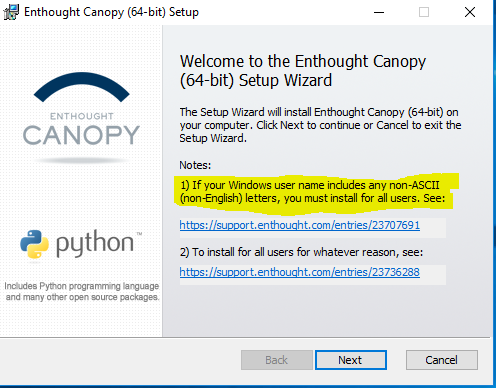
\includegraphics[width=1.0\textwidth]{figs/1.png}
%\end{figure}
%\begin{figure}
% 	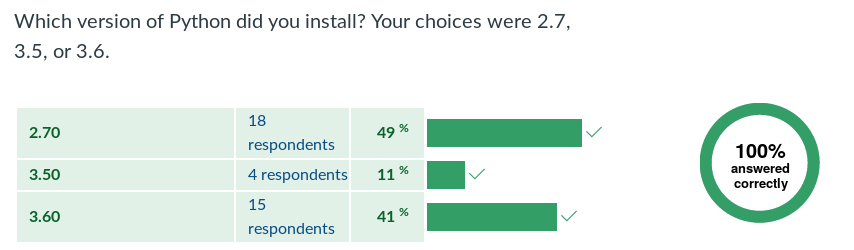
\includegraphics[width=1.0\textwidth]{figs/2.png}
%\end{figure}
%
%\end{frame}
%
%\begin{frame}{The operating systems used by the class}
%\begin{figure}
% 	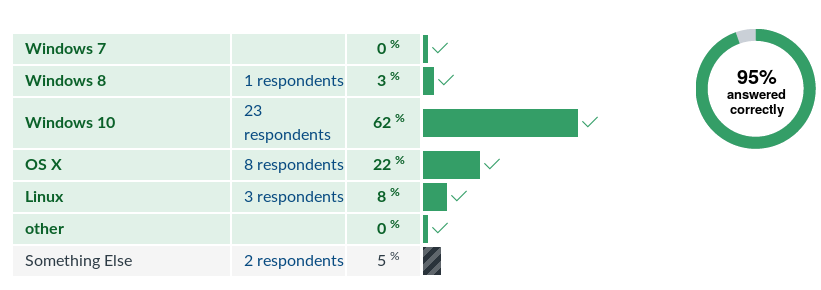
\includegraphics[width=1.0\textwidth]{figs/3.png}
%\end{figure}
%\end{frame}
%
%\begin{frame}{Textbook for this lecture}
%A whirlwind Tour of Python by Dr. VanderPlas is a short book to prepare users with the bare essentials
%for working with Python. 
%
%It is also available for free at
% \url{http://www.oreilly.com/programming/free/files/a-whirlwind-tour-of-python.pdf}
% 
% or \url{https://github.com/jakevdp/WhirlwindTourOfPython}
%  
%\end{frame}
%
%\begin{frame}[fragile]{Comments}
%\begin{minted}
%{python}
%# This is a comment in Python
%
%'''
%This is a bulk comment in python
%
%Any line between the start and the end
%
%is part of the comment
%'''
%
%\end{minted} 
%\end{frame}
%
%\begin{frame}[fragile]{Assigning variables}
%\begin{minted}
%{python}
%# Variables can be easily assigned
%# this code assigns integer 10 to x
%x = 10
%
%\end{minted}
%This officially defines a pointer named x that points to the integer 10. We can change what x points to at any time.
%\begin{minted}
%{python}
%x = 10      # x is the integer 10
%x = 10.     # x is the floating point EEE-754 double precision
%x = 10.0    # same as x = 10.
%x = 'ten'   # x is now a string
%x = (0,1,2) # x is now a tuple
%x = [0,1,2] # x is now a list
%x = 1; y = 2; z = 3 # assigns x = 1, y = 2, and z = 3
%\end{minted}
%\end{frame}
%
%\begin{frame}[fragile]{Demo - Consequences of pointers}
%\textbf{Be careful.} 
%\begin{minted}
%{python}
%x = [1,2,3]
%y = x
%x[0] = 4
%print(y)
%\end{minted}
%
%\textbf{Numpy warning!}
%\begin{minted}
%{python}
%import numpy as np
%x = np.array([10])
%y = x 
%x += 5 
%print(y)
%# this doesn't  happen if I used x = x + 5
%# this doesn't happen if x = 10 (instead of np.array([10]))
%\end{minted}
%\end{frame}
%
%\begin{frame}{Math operators}
%\begin{table}
%\begin{tabular}{lll}
%\textbf{Operater} & \textbf{Name} & \textbf{Description} \\
%\hline
%a + b & Addition & Sum of a and b \\
%a - b & Subtraction & Difference of a and b \\
%a * b & Multiplication & Product of a and b \\
%a / b & True division & Quotient of a and b \\
%a // b & Floor division & Quotient of a and b , removing fractional parts \\
%a \% b  & Modulus & Remainder after division of a by b \\
%a ** b & Exponentiation & a raised to the power of b \\
%-a & Negation & The negative of a \\
%+a & Unary & plus a unchanged (rarely used) \\
%\end{tabular}
%\end{table}
%
%Page 18 of A Whirlwind Tour of Python by VanderPlas.
%\end{frame}
%
%\begin{frame}[fragile]{Division in Python2}
%Let's take a look at division in Python2
%\begin{minted}
%{python}
%a = 3
%b = 2
%c = a/b
%\end{minted}
%So we have integer a divided by integer b and I'm familiar with programming so I expect c to be an integer. 
%\end{frame}
%
%\begin{frame}[fragile]{Python3 \textit{broke} division!}
%or \textit{Fixed} it, because in Python3 an integer divided by an integer magically becomes a float. Remember that import future command? We can use it to get Python3 division in Python2.
%\begin{minted}
%{python}
%from __future__ import division
%a = 3
%b = 2
%c = a/b
%\end{minted}
%\end{frame}
%
%\begin{frame}[fragile]{Built in data types}
%Here are the built in data types for Python. Use
%\begin{minted}
%{python}
%type(x)
%\end{minted}
%
%to display the data type of x.
%\begin{table}
%\begin{tabular}{lll}
%\textbf{Type} & \textbf{Example} & \textbf{Description} \\
%\hline
%int      & x = 1  &  Integers (i.e., whole numbers) \\
%float    & x = 1.0 & Floating-point numbers (i.e., real numbers) \\
%complex  & x = 1 + 2j & Complex numbers \\
%bool     & x = True & Boolean: True/False values \\
%str      & x = 'abc' & String: characters or text \\
%NoneType & x = None & Special object indicating nulls \\
%\end{tabular}
%\end{table}
%str(x) converts x to a string
%int(x) converts x to an integer
%float(x) converts x to a floating point
%
%Page 24 of A Whirlwind Tour of Python by VanderPlas.
%\end{frame}
%
%
%\begin{frame}[fragile]{Comparison operators}
%Comparison operators will return a boolean 
%\begin{minted}
%{python}
%True
%False
%\end{minted}
%\begin{table}
%\begin{tabular}{ll}
%\textbf{Operation} & \textbf{Description} \\
%\hline
%a == b & a equal to b \\
%a != b & a not equal to b \\
%a $<$ b  & a less than b \\
%a $>$ b  & a greater than b \\
%a $<=$ b & a less than or equal to b \\
%a $>=$ b & a greater than or equal to b \\
%\end{tabular}
%\end{table}
%Page 21 of A Whirlwind Tour of Python by VanderPlas.
%\end{frame}
%
%\begin{frame}[fragile]{Floating point precision}
%\begin{minted}
%{python}
%0.1+0.2 == 0.3
%\end{minted}
%this returns False! Why? 
%
%You can use the numpy isclose function to set a tolerance for floating point comparison.
%\end{frame}
%
%\begin{frame}{Data Structures}
%\begin{table}
%\begin{tabular}{lll}
%\textbf{Type Name} & \textbf{Example} & \textbf{Description} \\
%\hline
%list  & [1, 2, 3] & Ordered collection \\
%tuple & (1, 2, 3) & Immutable ordered collection \\
%dict  & \{'a':1, 'b':2, 'c':3\} & Unordered (key,value) mapping \\
%set   & \{1, 2, 3\} & Unordered collection of unique values \\
%\end{tabular}
%\end{table}
%Page 30-31 of A Whirlwind Tour of Python by VanderPlas.
%	\begin{alertblock}{Mutable}
%	Can be changed and modified
%	\end{alertblock}
%	\begin{alertblock}{Immutable}
%	Can not be changed or modified
%	\end{alertblock}
%\end{frame}
%
%\begin{frame}[fragile]{Lists are amazing}
%Lists
%\begin{itemize}
%\item basic \textbf{ordered} and \textbf{mutable} data collections
%\item Lists can be any shape and contain any data type
%\item you can have lists, floats, integers, tuple, dictionaries, sets in lists
%\item a float of 10.0 can be added to a list x by x.append(10.0)
%\item list x can be sorted by x.sort()
%\item the number of items in list x can be found with len(x)
%\end{itemize}
%\end{frame}
%
%\begin{frame}{Pimp my list}
%\begin{figure}
% 	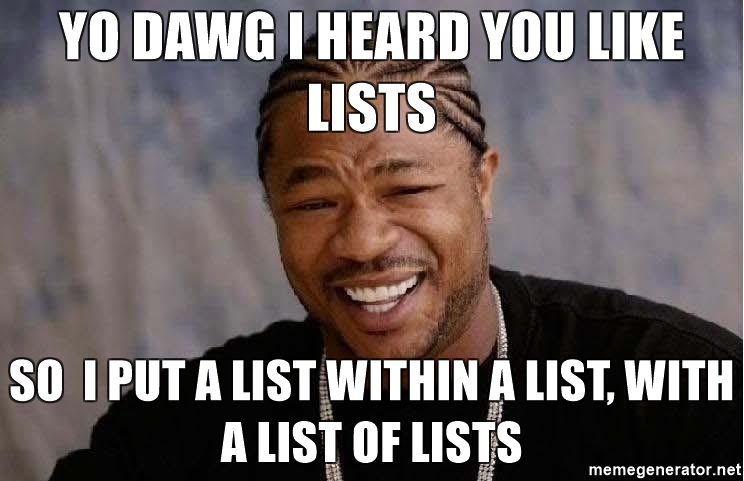
\includegraphics[width=1.0\textwidth]{figs/pimpmylist.jpg}
%\end{figure}
%\end{frame}
%
%\begin{frame}{Listception}
%\begin{figure}
% 	
\includegraphics[width=1.0\textwidth]{figs/listception.jpg}
%\end{figure}
%\end{frame}
%
%\begin{frame}[fragile]{An example list}
%\begin{minted}
%{python}
%x = [] # initialize an empty list
%x.append(0.0) # append float 0.0 to x
%x.append(1) # append integer 1 to x
%x.append([3,4,'hi',(10,8)]) # append a list with a tuple to x
%x.sort() # sort x from low to high 
%n = len(x) # count the number of items in list x
%print('There are ',n,' items in list x')
%print(x) 
%\end{minted}
%\textbf{Note}: x.sort() doesn't work in this case with Python 3 since you would need to compare different data types!!!
%\end{frame}
%
%\begin{frame}[fragile]{List forward indexing - lists start at 0}
%\begin{minted}
%{python}
%x = [7, 77, 777, 7777]
%\end{minted}
%The first item in the list can be called using
%\begin{minted}
%{python}
%in : x[0]
%out: 7
%\end{minted}
%The second item of the list can be called using
%\begin{minted}
%{python}
%in : x[1]
%out: 77
%\end{minted}
%The third item of the list can be called using 
%\begin{minted}
%{python}
%in : x[2]
%out: 777
%\end{minted}
%The last item of the list can be called using
%\begin{minted}
%{python}
%in : x[3]
%out: 7777
%\end{minted}
%\end{frame}
%
%\begin{frame}[fragile]{List backward indexing - last index item in Python is -1} 
%\begin{minted}
%{python}
%x = [7, 77, 777, 7777]
%\end{minted}
%The last item in the list can be called using
%\begin{minted}
%{python}
%in : x[-1] 
%out: 7777
%\end{minted}
%The second to last item of the list can be called using
%\begin{minted}
%{python}
%in : x[-2]
%out: 777
%\end{minted}
%The third to last item of the list can be called using 
%\begin{minted}
%{python}
%in : x[-3]
%out: 77
%\end{minted}
%The fourth to last item of the list can be called using
%\begin{minted}
%{python}
%in : x[-4]
%out: 7
%\end{minted}
%\end{frame}
%
%\begin{frame}[fragile]{List slicing}
%\begin{minted}
%{python}
%x = [7, 77, 777, 7777]
%\end{minted}
%List slicing is [startPoint : endPoint] where startPoint is inclusive and endPoint is exclusive. In Mathematics would define define the interval as [startPoint, endPoint).
%
%If we wanted the first and second item in a list
%\begin{minted}
%{python}
%in : x[0:2]
%out: [7, 77]
%\end{minted}
%
%So if we want the second through fourth item in list x
%\begin{minted}
%{python}
%in : x[1:4]
%out: [77, 777, 7777]
%\end{minted}
%\end{frame}
%
%\begin{frame}[fragile]{Slicing with step size}
%\begin{minted}
%{python}
%x = [0, 1, 2, 3, 4, 5, 6, 7, 8, 9,
%    10, 11, 12, 13, 14, 15,
%    16, 17, 18, 19] # creates a list of integers
%\end{minted}
%
%We can slice with [startPoint:endPoint:stepSize], just like before, but now stepSize is the step size of our slice. 
%
%\begin{minted}
%{python}
%in : x[0:20:2]
%out: [0, 2, 4, 6, 8, 10, 12, 14, 16, 18]
%\end{minted}
%
%\begin{minted}
%{python}
%in : x[0:20:5]
%out: [0, 5, 10, 15]
%\end{minted}
%
%\begin{minted}
%{python}
%in : x[1:20:3]
%out: [1, 4, 7, 10, 13, 16, 19]
%\end{minted}
%\end{frame}
%
%\begin{frame}[fragile]{Reverse the order of a list}
%Sometimes it is useful to reverse the order of a list. We can do this by consider a backwards slice.
%\begin{minted}
%{python}
%x = [7, 77, 777, 7777]
%\end{minted}
%
%So to see the reverse order of x we would run
%\begin{minted}
%{python}
%in : x[::-1]
%out: [7777, 777, 77, 7]
%\end{minted}
%\end{frame}
%
%
%
%\begin{frame}[fragile]{Tuples}
%Tuples are just like lists, except you define a tuple with parentheses instead of square brackets. List indexing a slicing of Tuples works exactly like lists, and you'll use square brackets to call items of a tuple.
%
%\textbf{Tuples are immutable} which means that once they are created they can't be modified in any way. I hardly ever use Tuples.
%
%Let's create a tuple of 2, 4, 6.
%\begin{minted}
%{python}
%x = (2, 4, 6)
%\end{minted}
%
%\begin{minted}
%{python}
%in : x[0]
%out: 2
%\end{minted}
%
%
%\begin{minted}
%{python}
%in : x[-1]
%out: 6
%\end{minted}
%
%
%\end{frame}
%
%\begin{frame}[fragile]{Dictionaries}
%Dictionaries map keys to values. There is no index with dictionaries, instead there is a key. Dictionaries are sometimes used to pass parameters into a function.
%
%Let's take a look at this param dictionary for the XGDBoost library as an example dictionary. \url{http://xgboost.readthedocs.io/en/latest/python/python_intro.html}
%
%\begin{minted}
%{python}
%param = {'max_depth':2, 'eta':1, 'silent':1,
% 'objective':'binary:logistic' }
%param['nthread'] = 4
%param['eval_metric'] = 'auc'
%\end{minted}
%
%We don't can add keys to the dictionary at any time! Let's take a look at param.
%\begin{minted}
%{python}
%in : print(param)
%out: {'silent': 1, 'eval_metric': 'auc', 'nthread': 4,
% 'eta': 1, 'objective': 'binary:logistic', 'max_depth': 2}
%\end{minted}
%
%\end{frame}
%
%\begin{frame}[fragile]{Dictionaries - param continued}
%Find values of keys with square brackets.
%\begin{minted}
%{python}
%in : param['objective']
%out: 'binary:logistic'
%\end{minted}
%
%We can easily assign a new value for a key
%\begin{minted}
%{python}
%in : param['objective'] = 'reg:linear'
%in : print(param['objective'])
%out: 'reg:linear'
%\end{minted}
%\end{frame}
%
%\begin{frame}[fragile]{Sets}
%Sets are like lists and tuples, but are defined with curly brackets. Sets obey mathmatical set definitions. VanderPlas provides a good example on page 36-37. Which I'll show here.
%\begin{minted}
%{python}
%in : primes = {2, 3, 5, 7}; odds = {1, 3, 5, 7, 9}
%in : primes.union(odds) # union of primes and odds
%out: {1, 2, 3, 5, 7, 9}
%in : primes.intersect(odds) # intersection of primes and odds
%out: {3, 5, 7}
%in : primes.difference(odds) # items in primes but not odds
%out: {2}
%in : primes.symmetric_difference(odds) # items in just one set
%out: {1, 2, 9}
%\end{minted}
%\end{frame}
%
%
%\begin{frame}{Membership operator}
%\begin{table}
%\begin{tabular}{ll}
%\textbf{Operator} & \textbf{Description} \\
%\hline
%a is b     & True if a and b are identical objects \\
%a is not b & True if a and b are not identical objects \\
%a in b     & True if a is a member of b \\
%a not in b & True if a is not a member of b \\
%\end{tabular}
%\end{table}
%Page 23 of A Whirlwind Tour of Python by VanderPlas.
%\end{frame}
%
%\begin{frame}[fragile]{If-then statements}
%Let's take a look at a if, elif, and else statement in Python.
%
%\begin{minted}
%{python}
%x = 9
%if x < 0:
%    print(x,' is a negative number')
%elif x > 0:
%    print(x,' is a positive number')
%elif x == 0:
%    print('Single')
%else:
%    print(x,' makes me confused!')
%\end{minted}
%
%This obviously returns
%(9, ' is a positive number')
%
%\end{frame}
%
%\begin{frame}[fragile]{If-then statements - notes}
%\begin{minted}
%{python}
%x = 9
%if x < 0:
%    print(x,' is a negative number')
%elif x > 0:
%    print(x,' is a positive number')
%elif x == 0:
%    print('Single')
%else:
%    print(x,' makes me confused!')
%\end{minted}
%
%\begin{itemize}
%\item in Python code blocks are denoted by indentation
%\item remember the emphasis on Python is to create highly readable code
%\item by forcing you to indent your code block
%\item the recommendation is that you use four spaces to denote an indent
%\item but you can also use tab
%\item indentations are preceded by a :
%\end{itemize}
%
%\end{frame}
%
%\begin{frame}[fragile]{Subsequent code blocks are also indented}
%\begin{minted}
%{python}
%x = 9
%if x > 0:
%    print(x,' is a greater than zero')
%    if x > 5:
%        print(x,' is a greater than five')
%        if x > 10:
%            print(x,' is greater than 10')
%    # this is the continued x > 0 code block
%    print('the date type of x is ', type(x))
%\end{minted}
%
%Note that this will print the type of x only when x $>$ 0!
%\end{frame}
%
%\begin{frame}{tabs vs spaces}
%In a survey it was found that those who use spaces make more money
%\url{https://stackoverflow.blog/2017/06/15/developers-use-spaces-make-money-use-tabs/}
%\begin{figure}
% 	
\includegraphics[width=1.0\textwidth]{figs/money.jpg}
%\end{figure}
%\end{frame}
%
%\begin{frame}{tabs vs spaces}
%\begin{figure}
% 	
\includegraphics[width=0.6\textwidth]{figs/tabsVSpaces.jpg}
%\end{figure}
%\end{frame}



%\begin{frame}[fragile]{HW 01 - turn in one week from today in Canvas}
%Turn in the 5 questions as a single .py file onto canvas. Use comments to clearly indicate which question you are working on. Your filename should end as \_py2.py if you use Python2 and \_py3.py if you use Python3.
%\begin{enumerate}
%\item Name one difference between Python2 and Python3. Print your answer as a string in Python.
%\item You are given a list x = [0,1,2,3,4,5,6]. Print the third item in list x.
%\item Assign y as the reversed order of list x. Print y.
%\item Use list slicing to assign z [1,3,5] from x. Print z.
%\item Your friend is new to Python. He is confused why his if statement isn't working, he has a number x and wants to print 'x is positive' by checking with an if statement.  His code is following.
%\begin{minted}
%{python}
%x = 99
%if (x > 0) is True
%print('x is positive')
%\end{minted}
%This returns an 'invalid syntax error'. Copy this code into your .py file, and correct the code.
%\end{enumerate}
%
%\end{frame}

%\begin{frame}[fragile]{HW 01 - turn in one week from today in Canvas}
%\begin{enumerate}
%\setcounter{enumi}{5}
%\item The Fibonacci sequence is defined as
%\begin{equation}
%F_n = F_{n-1} + F_{n-2}
%\end{equation}
%where $n$ denotes the $n^\text{th}$ item of the Fibonacci sequence. You are given the first three numbers of the Fibonacci sequence as F = [0, 1, 1]. Create a for loop to determine the next 20 numbers of the Fibonacci sequence. Print F with the final 23 numbers. Hint: use F.append() to add a new Fibonacci value to the end of the list F.
%\item Parentheses are used to preserve order of operations in Python. The following code will add x+y first, then raise to the power z. This value is assigned g.
%\begin{minted}
%{python}
%g = (x+y)**z
%\end{minted} 
%Given the list x = [2.0,3.0,5.0,7.0,9.0], create a list $Y(x)$ for each float in x. Print the list $Y$.
%\begin{equation}
%Y(x) = \frac{(3.0x)^2}{(99x - x^3)} - \frac{1}{x}
%\end{equation} 
%\end{enumerate}
%
%\end{frame}

%\begin{frame}{About me}
%PhD Student in the MDO lab. 
%
%I look at improving techniques for selecting material parameters.
%
%My interests:
%\begin{itemize}
%\item non-linear finite element (FE) method
%\item non-linear material modeling
%\item inverse analysis
%\item optimization
%\item regression and classification
%\item digital image correlation (DIC)
%\item high performance computing (HPC)
%\item Python
%\end{itemize}
%
%For more see \url{http://jekel.me}
%
%\end{frame}
%
%\begin{frame}{About the course}
%Syllabus available online.
%
%The intention of this course is to prepare you to for doing numerical work in Python.
%
%Course expectations:
%\begin{itemize}
%\item 12 out of 14 homework | 60~\%
%\item 2 quizzes | 10~\%
%\item 1 final exam | 30~\%
%\end{itemize}
%
%
%\end{frame}
%
%\begin{frame}{Intended audience}
%	\begin{alertblock}{Course description}
%Python is a general purpose programming language. Course covers the basics, linear algebra, plotting, and more to prepare students for solving numerical problems. Prerequisite: COP 2271 MATLAB or equivalent.
%	\end{alertblock}
%
%\textbf{You already know how to program in some language. \\
%You are interested in doing numerical analysis in Python.} 
%\end{frame}
%
%\begin{frame}{What is Python? - python.org}
%Let's see what \url{http://python.org} has to say about Python.
%      	
%      	\begin{figure} 	
% 	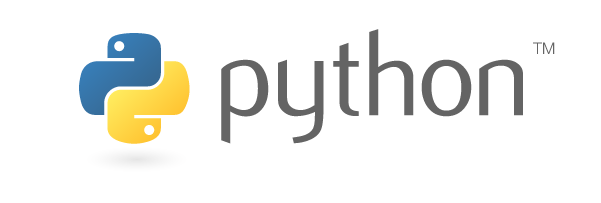
\includegraphics[width=0.65\textwidth]{figs/pythonLogo.png}
%      \end{figure}
%
%\textbf{Python is}
%\begin{itemize}
%\item an interpreted, object-oriented, high-level programming language with dynamic semantics
%\item very attractive for Rapid Application Development
%\item a simple and easy to learn syntax
%\end{itemize}
%\end{frame}
%
%\begin{frame}{Python is a very popular programming language}
%For the first time ever, IEEE Spectrum rated Python the most popular programming language in 2017. \url{http://spectrum.ieee.org/computing/software/the-2017-top-programming-languages}
%\begin{figure}
% 	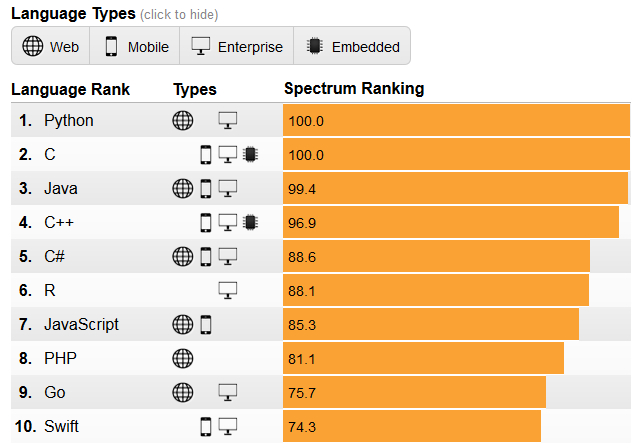
\includegraphics[width=0.85\textwidth]{figs/ieee.png}
%\end{figure}
%\end{frame}
%
%\begin{frame}{Built using Python}
%\begin{figure}
%
\includegraphics[width=1.0\textwidth]{figs/logos.png}
%\end{figure}
%\end{frame}
%
%\begin{frame}{Why Python? - Free, Open, and Powerful}
%  \begin{columns}[onlytextwidth]
%    \column{0.7\textwidth}
%\begin{itemize}
%\item Python is Free and Open
%\item Python can be used commercially 
%\item From research to deployment
%\item Libraries to do everything
%\item Adapted by scientist and engineers
%\item Cross platform support
%\end{itemize}
%    \column{0.3\textwidth}
%          \begin{figure} 	
% 	
\includegraphics[width=1.0\textwidth]{figs/free-beer.jpg}
%      \end{figure}
%  \end{columns}
%\end{frame}
%
%\begin{frame}{Python2 vs Python3}
%There is a syntax difference between Python version 2 and Python version 3. 
%
%When Python 3.0 was released in 2008 it broke backwards compatibility with Python 2.X. This was a mistake, and resulted in a very slow adaption of Python 3. 
%
%There are likely Python libraries that have yet to be ported to Python3. 
%
%Additionally there are libraries that were only written in Python3. 
%
%All new code should probably be written in a Python3 syntax, but I won't force you to use Python3. I still primarily use Python~2.7. Choose your version based on your library needs.
%
%For more see: \url{https://wiki.python.org/moin/Python2orPython3}
%\end{frame}
%
%\begin{frame}{Python2 vs Python3 comparison}
%  \begin{columns}[onlytextwidth]
%    \column{0.5\textwidth}
%\textbf{Python2 wins}
%\begin{itemize}
%\item Speed - Python 2.7 will always be faster
%\item Legacy
%\item Python updates won't break your code!
%\end{itemize}
%    \column{0.5\textwidth}
%\textbf{Python3 wins}
%\begin{itemize}
%\item Unicode identifiers
%\item Strings unicode by default
%\item Simple matrix multiplication with @
%\end{itemize}
%  \end{columns}
%\end{frame}
%
%\begin{frame}{TensorFlow and Windows - you need Python 3.5}
%\begin{figure}
%
\includegraphics[width=0.5\textwidth]{figs/tf.png}
%\end{figure}
%If you are intested in using \textbf{TensorFlow on Windows,} you must use a very specific version of Python. 
%
%TensorFlow is a state-of-the-art machine learning library. 
%
%See \url{https://www.tensorflow.org/install/install_windows}
%\end{frame}
%
%\begin{frame}{Ways to run Python}
%Here is the Python2 hello world program saved as helloWorld2.py
%\inputminted{python}{code/helloWorld2.py}
%
%
%These are some of the ways to run Python.
%\begin{itemize}
%\item from an IDE (integrated development environment)
%\item python
%\item python helloWorld2.py
%\item ipython
%\item (while in IPython) \%run helloWorld2.py
%\item ipython qtconsole (qtconsole has added benefits)
%\item ipython notebook
%\end{itemize}
%\end{frame}
%
%\begin{frame}{python3 helloWorld2.py}
%Running this (helloWorld2.py) in Python3:
%\inputminted{python}{code/helloWorld2.py}
%gives me the following error:
%\begin{figure} 	
% 	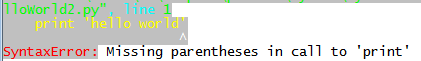
\includegraphics[width=1.0\textwidth]{figs/print23.png}
%\end{figure}
%because in Python3 \textit{print} is now a function
%\end{frame}
%
%\begin{frame}{python3 helloWorld3.py}
%With Python 3.X \textit{print} must include an open and closed parentheses. 
%
%The following code is saved as helloWorld3.py
%\inputminted{python}{code/helloWorld3.py}
%
%You can run this code with both python2 and python3.
%\end{frame}
%
%\begin{frame}{If you want to write code for Python 2.7 and Python 3.X}
%Your *.py script should always begin with these first three lines. The following code was saved as helloWorld.py.
%\inputminted{python}{code/helloWorld.py}
%This code runs with both python2 and python3. 
%\end{frame}
%
%\begin{frame}{Using future will force you to write in the Python 3.X syntax}
%Executing the following in python2
%\inputminted{python}{code/helloWorldBroke.py}
%Will give you an error!
%\end{frame}
%
%\begin{frame}{Python 3.X allows you to use unicode identifiers}
%\'{e} is a unicode character which can be used in the identifier (as a variable) in Python~3.X but not Python~2.X.
%
%Additionally strings in Python~3.X default to unicode (not the case in Python~2.X).
%
%The following code will only run in python3 (unicode breaks my syntax highlighting...)
%
%Fr\'{e}chet = 'Fr\'{e}chet is famous a French mathematician'
%
%print(Fr\'{e}chet)
%
%\end{frame}
%
%\begin{frame}{Comparing strings to numbers in Python 2 is weird}
%The following is input and output with python2 (it is not suppose to make any sense). 
%\mint{python}|'123' > 900|
%True
%\mint{python}|'123' > 0|
%True
%\mint{python}|'123' < 900|
%False
%\mint{python}|'123' < 0|
%False
%
%\textbf{Do not compare different data types in Python 2.X!}
%\end{frame}
%
%\begin{frame}{Python 3.X fixes string to number comparison}
%by not letting you compare data types that don't make sense
%\begin{figure}
% 	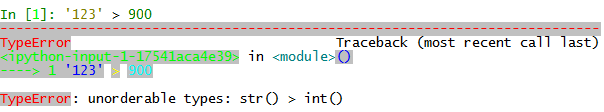
\includegraphics[width=1.0\textwidth]{figs/stringToIntPython3.png}
%\end{figure}
%\end{frame}
%
%\begin{frame}{Python 2.7 vs Python 3.X depends on you}
%Syntax differences:
%\begin{itemize}
%\item Python 3.X requires print to use parentheses
%\item In Python 3.X print is a function
%\item You can access the print function of Python~3.X in Python~2.7 by importing \textit{Future print function}
%\end{itemize}
%
%
%Additional resources:
%\begin{itemize}
%\item \url{http://python-future.org/imports.html}
%\item \url{https://wiki.python.org/moin/Python2orPython3}
%\item \url{https://learntocodewith.me/programming/python/python-2-vs-python-3/}
%\end{itemize}
%
%No more time for Python 2.7 vs Python 3.X. Pick one. Everything we do in this course will be compatible in both versions. You're allowed to use the version that best suits you. 
%\end{frame}
%
%\begin{frame}{Install python - do not install from \url{https://python.org}}
%Python builds from \url{https://www.python.org/downloads/} do not include pre-built libraries for numerical and scientific work. Compiling and building libraries is very complicated on Windows (and slightly less complicated on other operating systems). Think of this download as Python with no libraries.
%
%\textbf{DO NOT DOWNLOAD, DO NOT INSTALL.}
%\begin{figure}
% 	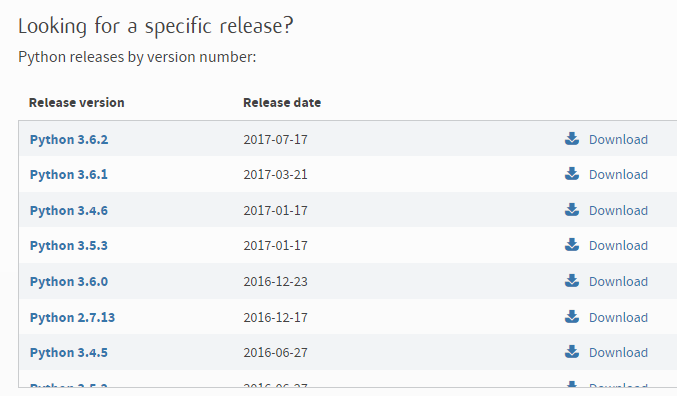
\includegraphics[width=1.0\textwidth]{figs/pythonVer.png}
%\end{figure}
%\end{frame}
%
%\begin{frame}{Install Python - two choices}
%For numerical and scientific work I recommend installing Anaconda or Enthought Canopy. These installations include the most popular libraries that are pre-built for your system. (I prefer Canopy, but use both.)
%  \begin{columns}[onlytextwidth]
%    \column{0.5\textwidth}
%          \begin{figure} 	
% 	
\includegraphics[width=1.0\textwidth]{figs/anaconda_logo.png}
%
%      \end{figure}
%    \column{0.5\textwidth}
%          \begin{figure} 	
% 	
\includegraphics[width=1.0\textwidth]{figs/canopy-logo.png}
%
%      \end{figure}
%  \end{columns}
%  
% Only a few months ago did Canopy start support Python~3.X, while Anaconda has supported Python~3.X for some time. I don't like Spyder IDE included with Anaconda because you can't bind crt + / to comment..
%\end{frame}
%
%\begin{frame}{Install Anaconda if ...}
%You want
%\begin{itemize}
%\item automatic environmental variable setup
%\item to have it your way
%\item to run multiple Python versions
%\item install TensorFlow or other ML libraries on Windows
%\item the powerful conda console tool for installing libraries
%\item the latest and greatest Python libraries
%\item Spyder IDE
%\end{itemize}
%
%\end{frame}
%
%\begin{frame}{Install Enthought Canopy if ...}
%You want
%\begin{itemize}
%\item the easiest Python scientific environment
%\item a pretty GUI for library management and updates
%\item Canopy IDE
%\item to add your Python environment variables manually
%\end{itemize}
%
%\end{frame}
%
%\begin{frame}{If you are coming from MATLAB ...}
%\textbf{Useful resources}
%\url{http://mathesaurus.sourceforge.net/matlab-numpy.html}
%\url{https://docs.scipy.org/doc/numpy-dev/user/numpy-for-matlab-users.html}
%\end{frame}
%
%\begin{frame}{Install Python - Anaconda}
%Anaconda gives you more control over which Python version. Also Anaconda updates more frequently.
%\url{https://www.continuum.io/downloads}
%          \begin{figure} 	
% 	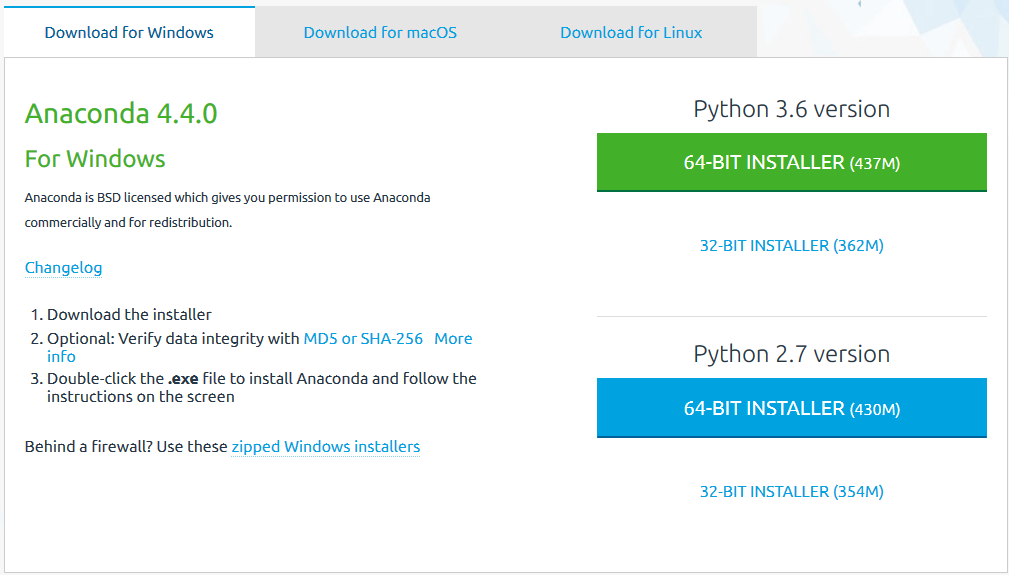
\includegraphics[width=1.0\textwidth]{figs/anaconda.png}
%      \end{figure}
%\end{frame}
%
%\begin{frame}{Anaconda - you should check these boxes}
%Unless you know how to manually edit the PATH environment variables
%\begin{figure}
% 	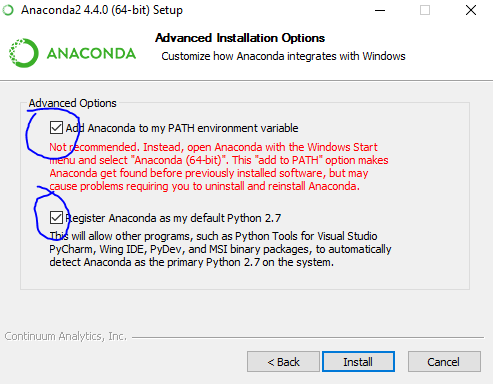
\includegraphics[width=0.85\textwidth]{pythonInstall/anacondaCheck.png}
%\end{figure}
%\end{frame}
%
%\begin{frame}{Spyder IDE installed with Anaconda}
%          \begin{figure} 	
% 	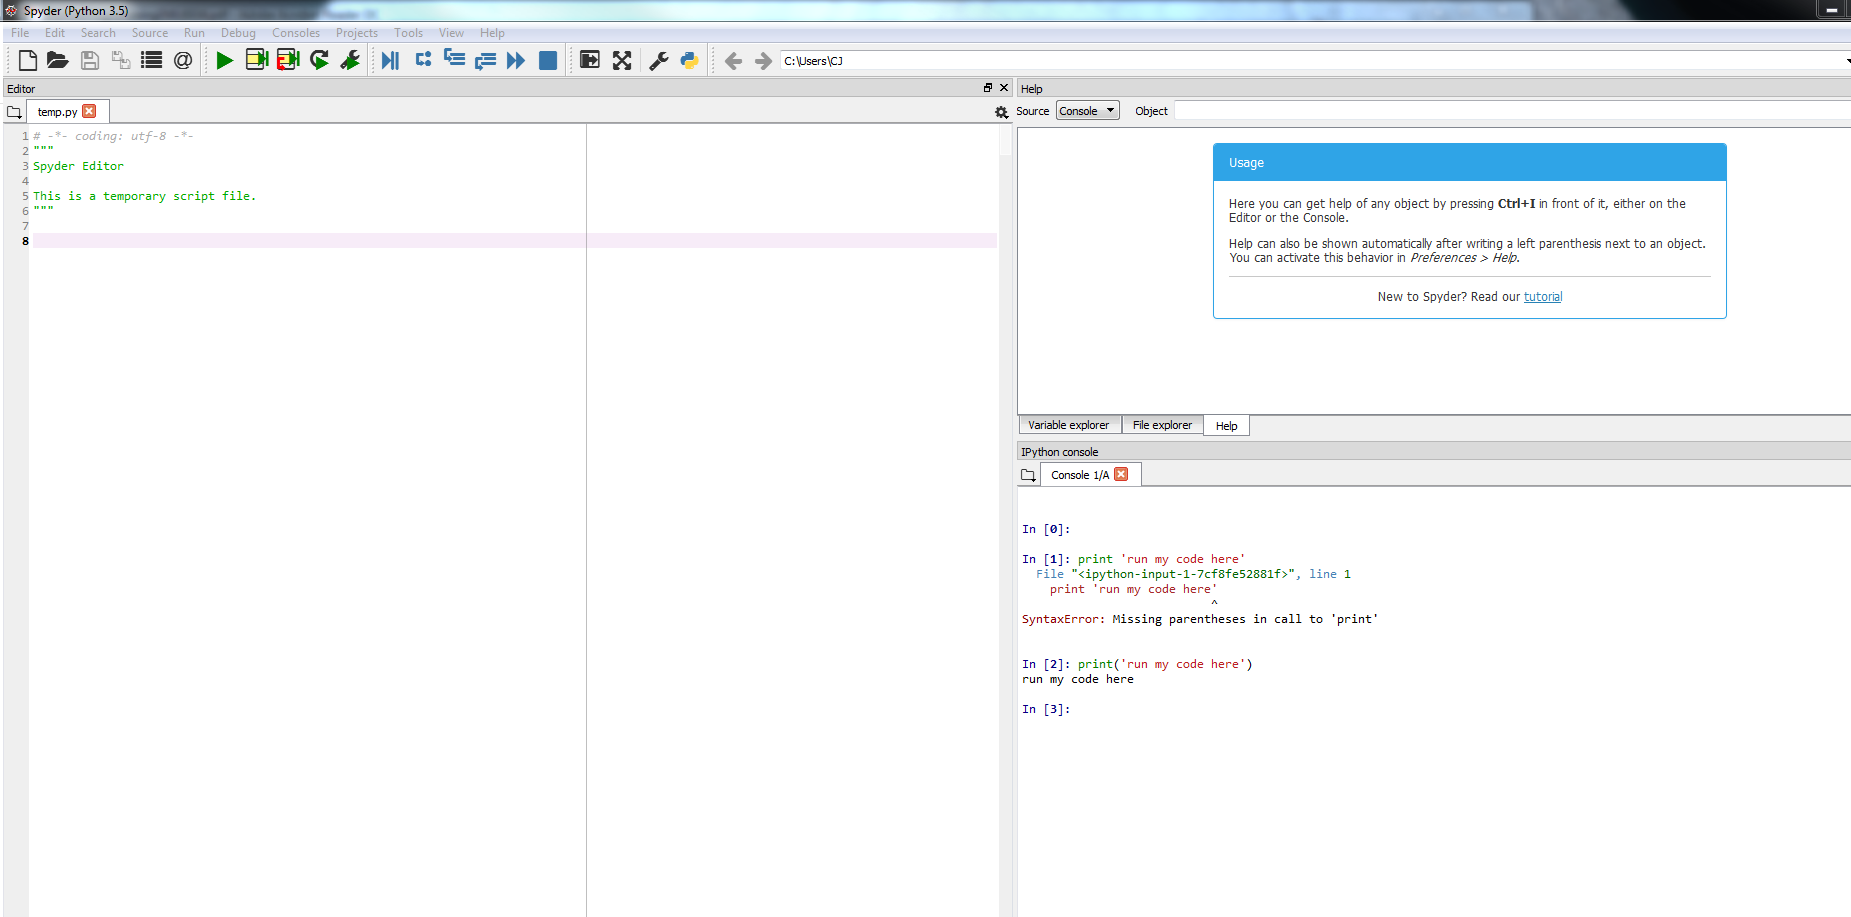
\includegraphics[width=1.0\textwidth]{figs/spyder.png}
%      \end{figure}
%\end{frame}
%
%\begin{frame}{Install Python - Enthought Canopy}
%With Enthought Canopy you may either install Python~2.7 or Python~3.5
%\url{https://store.enthought.com/downloads/}
%          \begin{figure} 	
% 	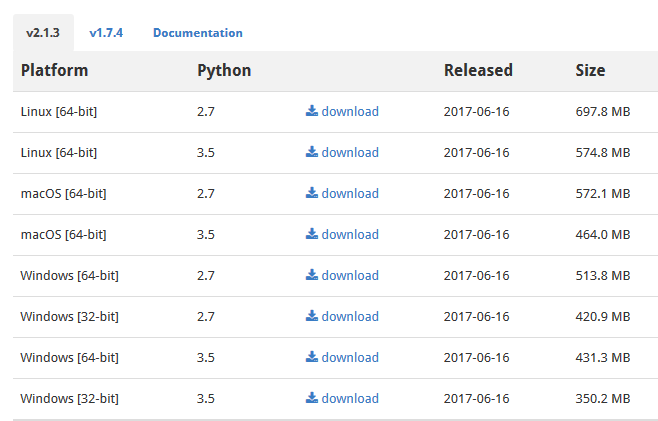
\includegraphics[width=1.0\textwidth]{figs/canopyInstall.png}
%      \end{figure}
%\end{frame}
%
%\begin{frame}{Canopy no longer sets up your environment variables by default...}
%You should add the following directories to your Path environment variable
%
%%\url{C:\Users\yourUserNameHere\AppData\Local\Enthought\Canopy\edm\envs\User}
%%\url{C:\Users\yourUserNameHere\AppData\Local\Enthought\Canopy\edm\envs\User\scripts}
%
%On Windows 7, 8, and 10 go to System $>$ Advanced System Settings $>$ environment variables.
%
%In Windows environment variables are separated without spaces using ;
%
%(If you didn't check the boxes with Anaconda, you'll need to set up the environment variables yourself)
%\end{frame}
%
%\begin{frame}{Canopy editor IDE installed with Enthought Canopy}
%          \begin{figure} 	
% 	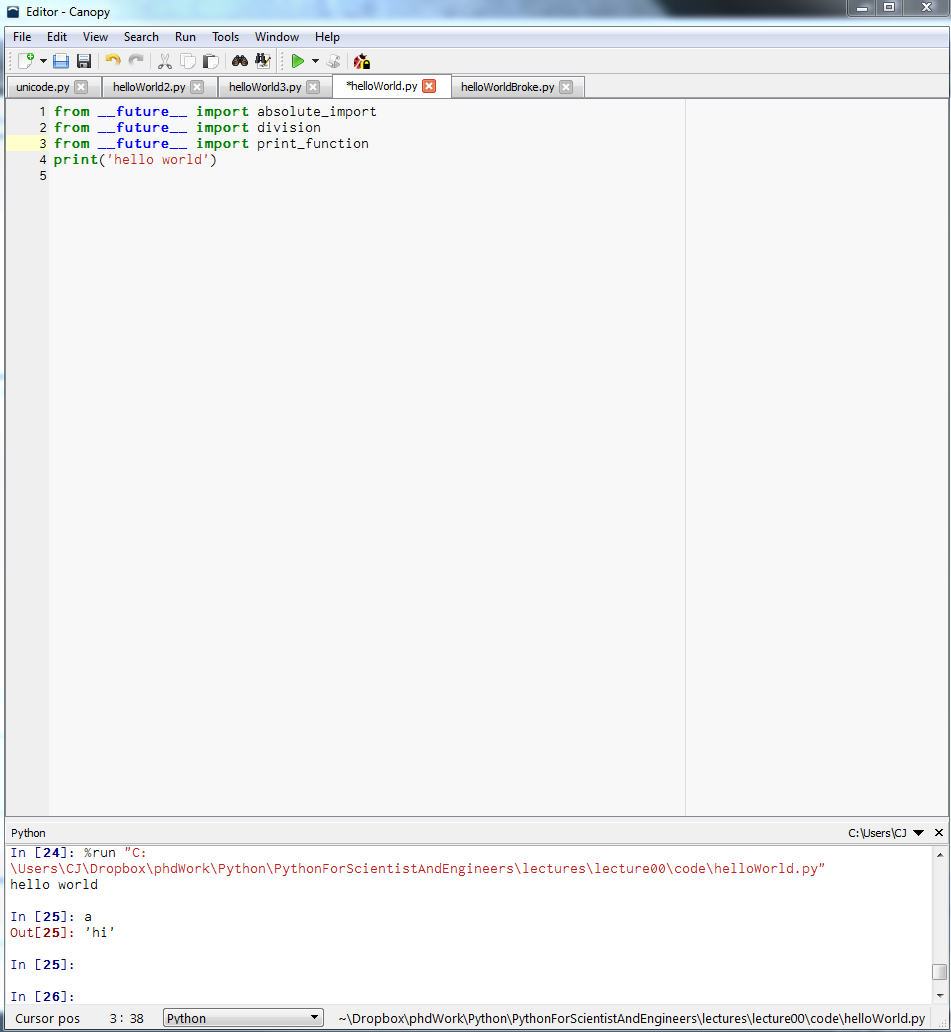
\includegraphics[width=.75\textwidth]{figs/canopy.png}
%      \end{figure}
%\end{frame}
%
%
%\begin{frame}{Anaconda vs Enthought Canopy doesn't matter for this course}
%... but what does matter is that you have a working Python installation with pre-built scientific libraries.
%\end{frame}
%
%\begin{frame}{Make sure you can run Python}
%However you install Python, please make sure that you can run python from the command line by typing python in your favorite shell/command prompt.
%
%\begin{figure}
% 	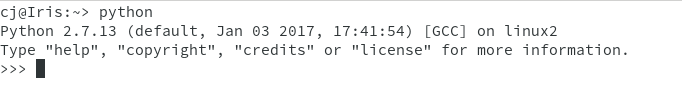
\includegraphics[width=1.0\textwidth]{figs/pythonLinux.png}
%\end{figure}
%
%On Windows (Open up a command prompt and type python followed by an enter). To open up a command prompt, hit the windows key and type command prompt. You should see a command prompt show up in the search.
%
%\end{frame}
%
%\begin{frame}{Also make sure that you can run pip}
%Also please ensure that you can run pip from your favorite shell/command prompt. 
%
%\begin{figure}
% 	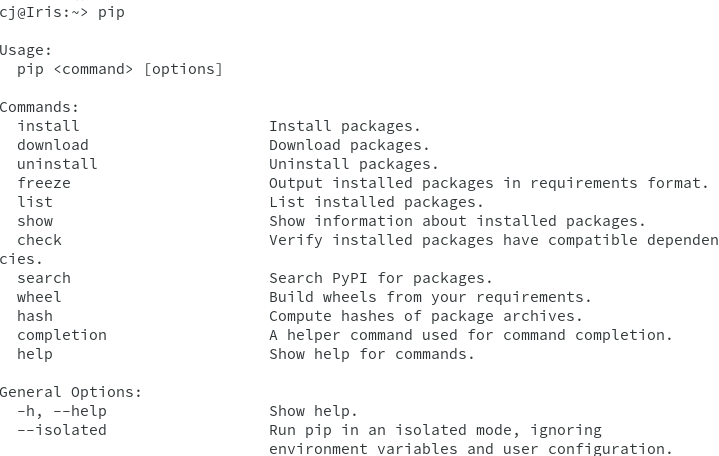
\includegraphics[width=1.0\textwidth]{figs/pipLinux.png}
%
%\end{figure}
%
%\end{frame}
%
%\begin{frame}{HW 00: due one week from today - turn in online before class starts}
%This HW will appear as a Quiz in Canvas. If you don't see the canvas Quiz please let me know!
%\begin{enumerate}
%\item Install Python. A) Tell me if you installed Anaconda or Enthought Canopy. B) Tell me which python version you installed (2.7, 3.5, 3.6?).
%\item What operating system do you use? (Ex: Windows 7, OS X Yosemite, Ubuntu 14)
%\item What previous programming languages are you familiar with? (Hint: only name the ones you have used the most)
%\end{enumerate}
%\end{frame}
%
%\begin{frame}{Tools used to make this presentation}
%This presentation was made with Beamer using \LaTeX. Texmaker is my favorite cross-platform \LaTeX ~editor. I use Metropolis, a modern Beamer theme. Syntax highlighting is done using Minted and Pygmentex. I use pdfpc (PDF presenter console) to present PDF files. 
%
%Links:
%\begin{itemize}
%\item \url{https://en.wikipedia.org/wiki/Beamer\_(LaTeX)}
%\item \url{https://www.latex-project.org/}
%\item \url{http://www.xm1math.net/texmaker/}
%\item \url{https://github.com/matze/mtheme}
%\item \url{https://www.ctan.org/pkg/minted?lang=en}
%\item \url{https://www.ctan.org/pkg/pygmentex?lang=en}
%\item \url{https://pdfpc.github.io/}
%\end{itemize} 
%
%\end{frame}






\end{document}
